%  !TeX spellcheck = en_GB
%  WangSheying于2015/11/2整理,TJU北洋园校区
%  TeXLive2015+TeXstudio个人推荐,可在线升级usepackage,比较方便
%*****************************************************************************************
%  从这里开始到\begin{document}是导言区,称之为preamble
\documentclass[UTF8]{beamer}
\usepackage[fontset=mac]{ctex}
%\usepackage[UTF8]{ctex}                 %使用中文要添加,可解决中文文档输入
\usepackage{newtxtext,newtxmath}  %字重齐全的高质量数学字体
\usepackage{mathrsfs}             %大写ABC的花体使用命令是\mathscr{}
\usepackage{graphicx}             %添加图片
\usepackage{bm}                   %专门处理数学粗体的bm宏包,使用命令是\bm{}
\usepackage{extarrows}            %延长符号,可在=,->等符号加多个字母
%\usepackage{amstext}              %它定义命令 \text,可用于在数学公式中插入少量文本,并可调整上下标中文本字体的尺寸。
\usepackage{amsthm}               %它定义了一个 proof 环境,用来排版定理和证明,能自动在最后添加证毕符号。它还提供一个命令:\newtheorem{定理环境名}{标题}[计数器名],可自定义定理类 环境
\usefonttheme{professionalfonts}  %这个更好看些,数学字体
\usepackage{indentfirst}          %首行缩进
\usepackage{amsmath}
\usepackage{amsfonts}
\usepackage{amssymb}
\usepackage{xcolor}
\usepackage{subfigure}
\usepackage[english]{babel}
\usepackage{algorithm}
\usepackage{algorithmic}
\usepackage{tikz}
\setlength{\parindent}{2em}      %首行缩进2字符
\setbeamertemplate{theorems}[numbered]
\setbeamertemplate{caption}[numbered]
%******************************************************************************************
%            以上是各种宏包
%******************************************************************************************
%下面是定理,定义,引言的声明,可自行添加

\newtheorem{thm}{Theorem}
%\newtheorem{lem}[thm]{Lemma}
\newtheorem{cor}[thm]{Corollary}
\newtheorem{prop}[thm]{Proposition}
\newtheorem{defi}[thm]{Definition}
\newtheorem{remark}[thm]{Remark}
\newtheorem{claim}[thm]{Claim}

\newenvironment{proofnoqed}{\begin{proof}<span style="background-color: rgb(255, 0, 0);">\renewcommand{\qedsymbol}{}  }{\end{proof} }
%有的证明比较长,前面的应该没有证毕符号,只在最后一个用proof,其他应该用自定义的新环境proofnoqed



%  三种颜色   red  purple   magenta





%上面是定理,定义,引言的声明,可自行添加
%******************************************************************************************
%下面是beamer的主题设置,目录框架结构,其实就是标题,目录等在上下左右哪一个位置放置,以及目录怎么显示
\usetheme{Singapore}            % 幻灯片模板选择singapore
\usecolortheme{sidebartab}      % 幻灯片模板的色彩sidebartab

\AtBeginSection[]{              % 幻灯片框架% 在每个Section前都会加入的Frame,
	\begin{frame}[plain]
		\frametitle{Outline}
		\tableofcontents[sectionstyle=show/shaded,subsectionstyle=show/show/shaded]
	\end{frame} 
}
%  \tableofcontents[comma-separated option list]具体讲解见《The beamer class User Guide》,
%  http://texdoc.net/texmf-dist/doc/latex/beamer/doc/beameruserguide.pdf     See in section 10.5 Adding a table of contents.
%  section和subsection相互独立,显示效果互不相关,Allowed ⟨styles⟩ are show, shaded, and hide
%  sectionstyle=⟨style for current section⟩/⟨style for other sections⟩
%  subsectionstyle=⟨style for current subsection⟩/⟨style for other subsections in current section⟩/⟨style for subsections in other sections⟩
%
% 上面是beamer的主题设置,目录框架结构,其实就是标题,目录等在上下左右哪一个位置放置,以及目录怎么显示
%*******************************************************************************************
%       下面标题页的内容设置,根据实际情况修改即可
\title{An Introduction to XGBoost}  % 幻灯片封面
\author{王社英}
\date{\today}  

%\date{9月 23, 2019}%一般是\today
%      上面标题页的内容设置根据实际情况修改即可
%*******************************************************************************************
%  \begin{document}以上是导言区,称之为preamble
%*******************************************************************************************
\begin{document}
	\begin{frame}[plain]
		%plain格式使得一帧的最上面是白色的,没有plain,会有色彩
		\titlepage
	\end{frame}
	\begin{frame}[plain]               % 幻灯片目录
		\frametitle{Outline}
		\tableofcontents[sectionstyle=show/show,subsectionstyle=show/show/hide]
	\end{frame}
	%The beamer class这本小册子有目录格式的讲解,sectionstyle,subsectionstyle都有,P100页
	%User Guide for version 3.36. 文档可在google搜索The beamer class,即可得到
%  以上是标准的配置,还有最下面的一部分标准配置
%********************************************************************************************
%    一帧的具体格式样例参考
%\section{节的名字}
%\subsection{小节的名字}
%\begin{frame}[plain,t]{节的名字} %也可以使用\frametitle{节的名字}效果一样
%	\structure{小节的名字} \\  \vspace{2ex}
%	节的名字正上方居中,小节的名字紧下方居左。
%\end{frame}
%*********************************************************************************************
%                  下面就是正文,自己的内容
%*********************************************************************************************

\section{XGBoost Introduction}
\begin{frame}[plain,t]{XGBoost Introduction} %也可以使用\frametitle{节的名字}效果一样
	   \vspace{2ex}
    
    XGBoost\cite{Chen2016XGBoost} is a scalable end to end tree boosting system.
    %it is used widely by data scientists to achieve state-of-the-art results
    %on many machine learning challenges.
    
    \vspace{2ex}
    
      
    \begin{itemize}
        
        \item a novel sparsity aware algorithm for sparse data
        
        \item weighted quantile sketch for approximate tree learning
        
        \item insights on cache access patterns, data compression and sharding
        
    \end{itemize}

\vspace{2ex}

    By combining these insights, XGBoost scales beyond billions
    of examples using far fewer resources than existing systems.
   \end{frame}




\section{Decision Tree Algorithm}
\subsection{ID3}
\begin{frame}[plain,t]{Decision Tree Algorithm} %也可以使用\frametitle{节的名字}效果一样
    \structure{ID3} \\  \vspace{2ex}
    Apache Spark is a unified analytics engine for large-scale data processing.
    
    
    
    
\end{frame}
\subsection{C4.5}
\begin{frame}[plain,t]{Decision Tree Algorithm} %也可以使用\frametitle{节的名字}效果一样
    \structure{C4.5} \\  \vspace{2ex}
    Apache Spark is a unified analytics engine for large-scale data processing.
    
    
    
    
\end{frame}
\subsection{CART}
\begin{frame}[plain,t]{Decision Tree Algorithm} %也可以使用\frametitle{节的名字}效果一样
    \structure{CART} \\  \vspace{2ex}
    Apache Spark is a unified analytics engine for large-scale data processing.
    
    
    
\end{frame}

\section{Gradient Boosting}
\subsection{Gradient Boosting}
\begin{frame}[plain,t]{Gradient Boosting} %也可以使用\frametitle{节的名字}效果一样
    \structure{Gradient Boosting} \\  
   
    \begin{figure}
        \centering
        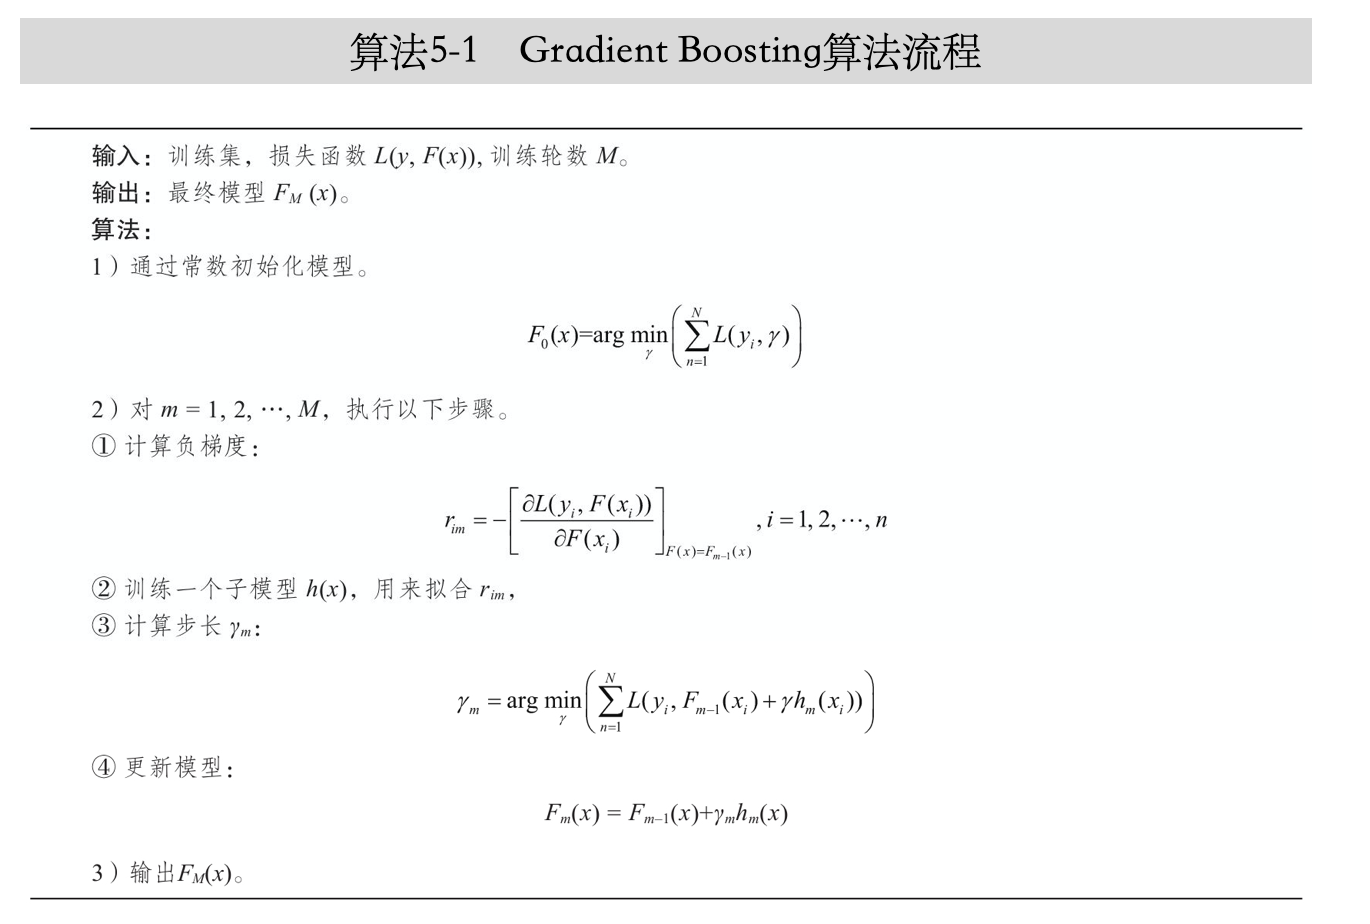
\includegraphics[width=0.9\linewidth]{images/gb1}
        %\caption{}
        \label{fig:gb1}
    \end{figure}
    
    
    
    
\end{frame}

\subsection{Gradient  Boosting Boosting}
\begin{frame}[plain,t]{Gradient Tree Boosting} 
    \structure{Gradient Tree Boosting\cite{xgbbook}} \\  
   \begin{figure}
       \centering
       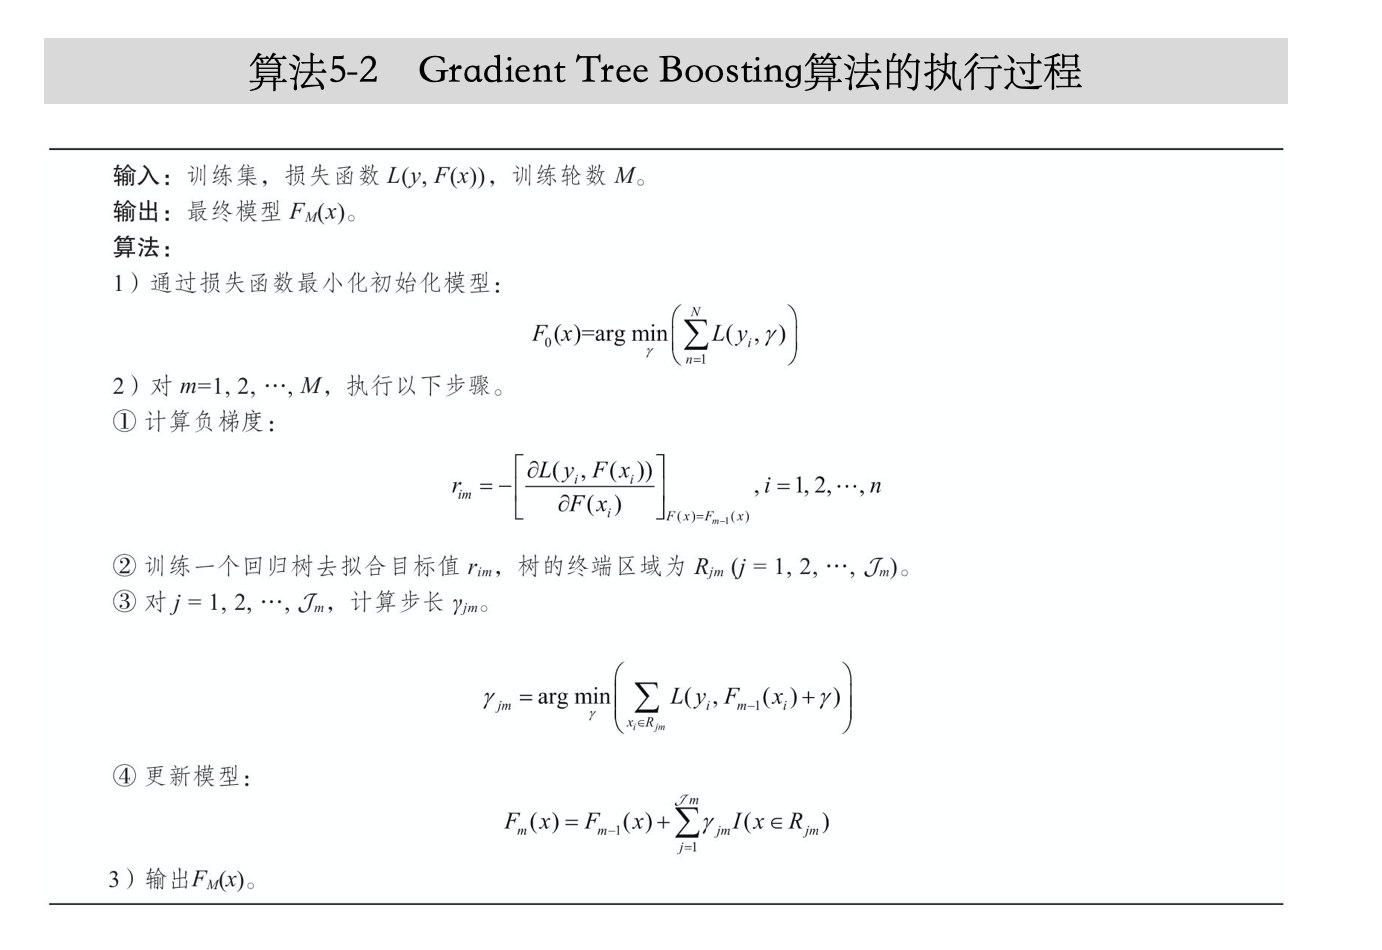
\includegraphics[width=0.9\linewidth]{images/gb2}
       %\caption{}
       \label{fig:gb2}
   \end{figure}
    
    
    
\end{frame}

\section{Tree Boosting}
\subsection{Additive Training}
\begin{frame}[plain,t]{Tree Boosting} %也可以使用\frametitle{节的名字}效果一样
    \structure{Additive Training} \\  \vspace{2ex}
    Apache Spark is a unified analytics engine for large-scale data processing.
    
    
    
    
\end{frame}

\subsection{Model Complexity}
\begin{frame}[plain,t]{Tree Boosting} %也可以使用\frametitle{节的名字}效果一样
    \structure{Model Complexity} \\  \vspace{2ex}
    Apache Spark is a unified analytics engine for large-scale data processing.
    
    
    
    
\end{frame}
\subsection{The Structure Score}
\begin{frame}[plain,t]{Tree Boosting} %也可以使用\frametitle{节的名字}效果一样
    \structure{The Structure Score} \\  \vspace{2ex}
    Apache Spark is a unified analytics engine for large-scale data processing.
    
    
    
    
\end{frame}

\subsection{Learn the tree structure}
\begin{frame}[plain,t]{Tree Boosting} %也可以使用\frametitle{节的名字}效果一样
    \structure{Learn the tree structure} \\  \vspace{2ex}
    Apache Spark is a unified analytics engine for large-scale data processing.
    
    
    
    
\end{frame}





%%=================================================================================================
\begin{frame}[plain]
    \huge
    \vfill
    \centerline{ \structure{Questions and Answers?} }
    \vfill
    
\end{frame}
\begin{frame}[plain]
    \huge
    \vfill
    \centerline{ \structure{Questions and Answers?} }
    \vfill
    \Huge
    \centerline{\alert{Thank You!} }
    \vfill
\end{frame}

%**********************************************************************************************
%                  上面就是正文,自己的内容
%        下面是标准的参考文献配置
%**********************************************************************************************
\begin{frame}[plain, t, allowframebreaks]{References}
    %  allowframebreaks,这个关键字可以使得参考文献自动断页,免得手动
    %  plain格式使得一帧的最上面是白色的,没有plain,会有色彩,可以试试
    %  t 使得正文不再是默认居中,而是在top,应该加上t,比较好看。
    \bibliographystyle{alpha}         %文献的格式apalike是[1],alpha是[Lam94]
    %\beamertemplatetextbibitems        %调整文献样式
    %\scriptsize                        %文献多时调整字体大小
    %\bibliography{math}                 %自己的文献
    \bibliography{xgb}
   
    
\end{frame}  
\end{document} 

